\documentclass[11pt,a4paper]{report}
\usepackage[textwidth=37em,vmargin=30mm]{geometry}
\usepackage{calc,xunicode,amsmath,amssymb,paralist,enumitem,tabu,booktabs,datetime2,xeCJK,xeCJKfntef,listings}
\usepackage{tocloft,fancyhdr,tcolorbox,xcolor,graphicx,eso-pic,xltxtra,xelatexemoji}

\newcommand{\envyear}[0]{2025}
\newcommand{\envdatestr}[0]{2025-07-09}
\newcommand{\envfinaldir}[0]{webdb/2025/20250709/final}

\usepackage[hidelinks]{hyperref}
\hypersetup{
    colorlinks=false,
    pdfpagemode=FullScreen,
    pdftitle={Web Digest - \envdatestr}
}

\setlength{\cftbeforechapskip}{10pt}
\renewcommand{\cftchapfont}{\rmfamily\bfseries\large\raggedright}
\setlength{\cftbeforesecskip}{2pt}
\renewcommand{\cftsecfont}{\sffamily\small\raggedright}

\setdefaultleftmargin{2em}{2em}{1em}{1em}{1em}{1em}

\usepackage{xeCJK,xeCJKfntef}
\xeCJKsetup{PunctStyle=plain,RubberPunctSkip=false,CJKglue=\strut\hskip 0pt plus 0.1em minus 0.05em,CJKecglue=\strut\hskip 0.22em plus 0.2em}
\XeTeXlinebreaklocale "zh"
\XeTeXlinebreakskip = 0pt


\setmainfont{Brygada 1918}
\setromanfont{Brygada 1918}
\setsansfont{IBM Plex Sans}
\setmonofont{JetBrains Mono NL}
\setCJKmainfont{Noto Serif CJK SC}
\setCJKromanfont{Noto Serif CJK SC}
\setCJKsansfont{Noto Sans CJK SC}
\setCJKmonofont{Noto Sans CJK SC}

\setlength{\parindent}{0pt}
\setlength{\parskip}{8pt}
\linespread{1.15}

\lstset{
	basicstyle=\ttfamily\footnotesize,
	numbersep=5pt,
	backgroundcolor=\color{black!5},
	showspaces=false,
	showstringspaces=false,
	showtabs=false,
	tabsize=2,
	captionpos=b,
	breaklines=true,
	breakatwhitespace=true,
	breakautoindent=true,
	linewidth=\textwidth
}






\newcommand{\coverpic}[2]{
    % argv: itemurl, authorname
    Cover photo by #2~~(\href{#1}{#1})
}
\newcommand{\makeheader}[0]{
    \begin{titlepage}
        % \newgeometry{hmargin=15mm,tmargin=21mm,bmargin=12mm}
        \begin{center}
            
            \rmfamily\scshape
            \fontspec{BaskervilleF}
            \fontspec{Old Standard}
            \fontsize{59pt}{70pt}\selectfont
            WEB\hfill DIGEST
            
            \vfill
            % \vskip 30pt
            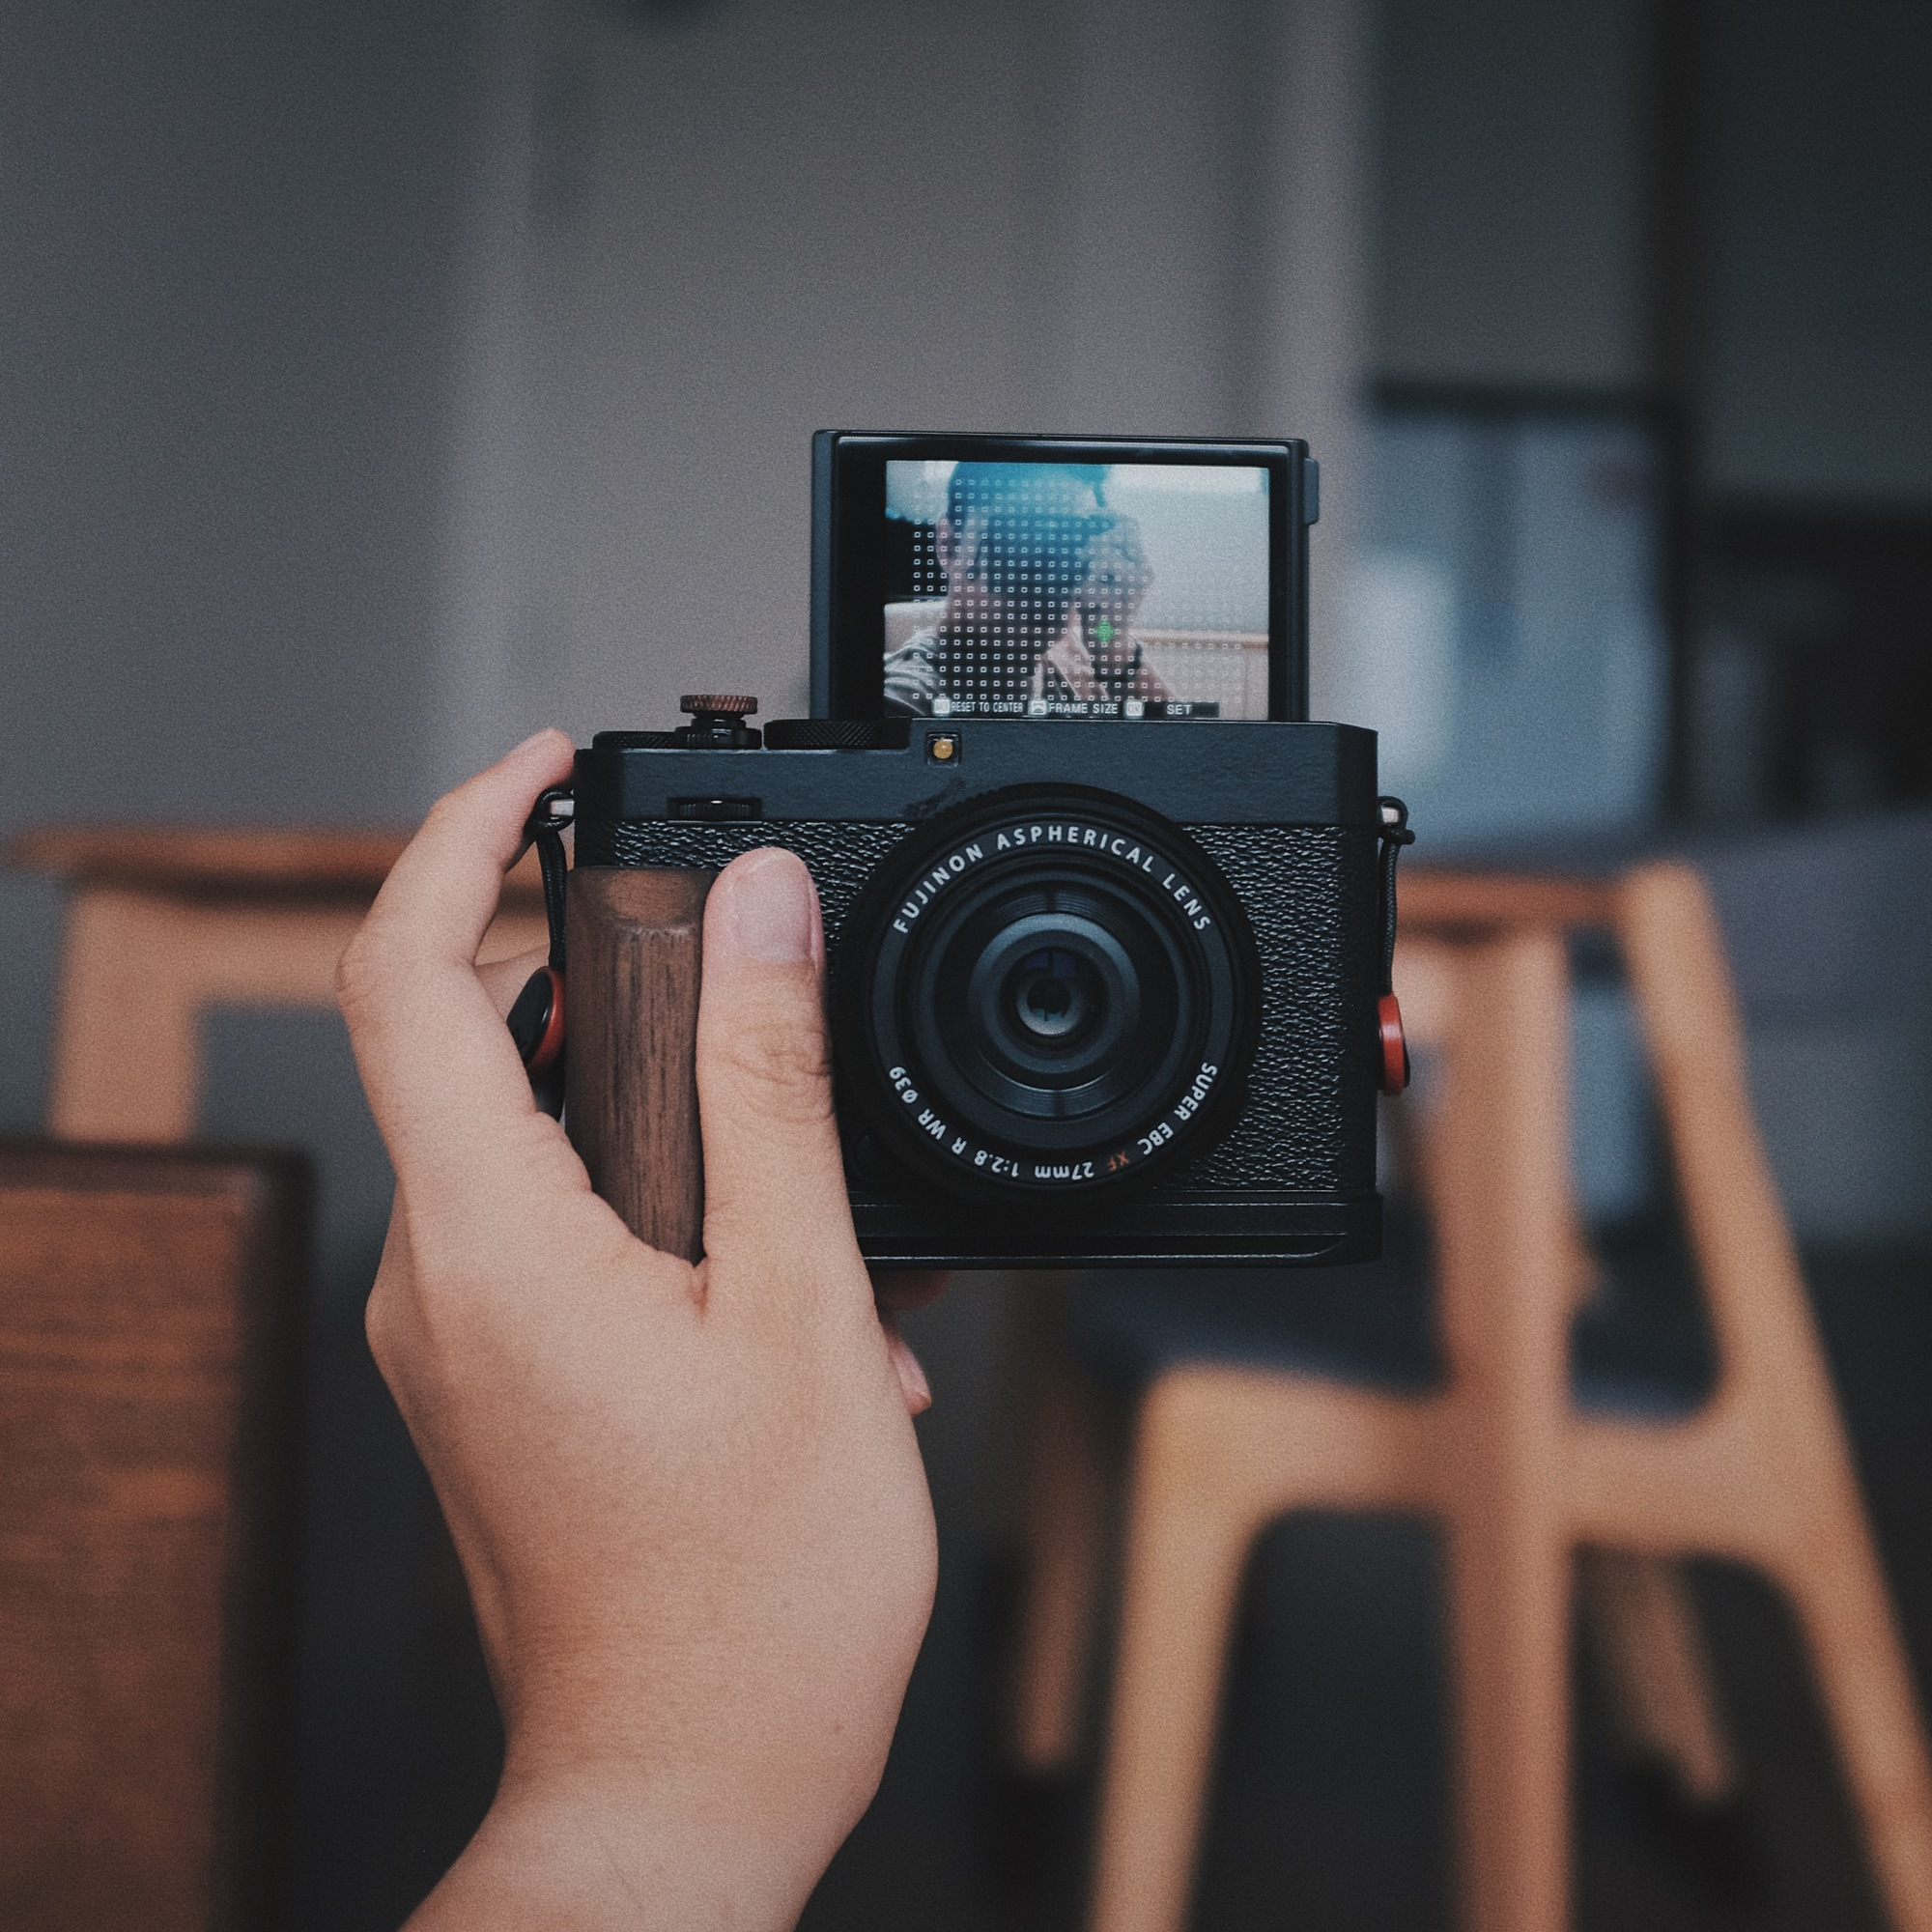
\includegraphics[width=\linewidth]{\envfinaldir/coverpic-prod.jpg}\par
            % \vskip 30pt
            \vfill

            \normalsize\rmfamily\scshape
            \copyright{} The Web Digest Project \hfill\large \envdatestr
        \end{center}
    \end{titlepage}
    % \restoregeometry
}
\newcommand{\simplehref}[1]{%
    \textcolor{blue!80!green}{\href{#1}{#1}}%
}
\renewcommand{\contentsname}{\center\Huge\sffamily\bfseries Contents\par\vskip 20pt}
\newcounter{ipartcounter}
\setcounter{ipartcounter}{0}
\newcommand{\ipart}[1]{
    % \vskip 20pt
    \clearpage
    \stepcounter{ipartcounter}
    \phantomsection
    \addcontentsline{toc}{chapter}{#1}
    % \begin{center}
    %     \Huge
    %     \sffamily\bfseries
    %     #1
    % \end{center}
    % \vskip 20pt plus 7pt
}
\newcounter{ichaptercounter}
\setcounter{ichaptercounter}{0}
\newcommand{\ichapter}[1]{
    % \vskip 20pt
    \clearpage
    \stepcounter{ichaptercounter}
    \phantomsection
    \addcontentsline{toc}{section}{\numberline{\arabic{ichaptercounter}}#1}
    \begin{center}
        \Huge
        \sffamily\bfseries
        #1
    \end{center}
    \vskip 20pt plus 7pt
}
\newcommand{\entrytitlefont}[1]{\subsection*{\raggedright\Large\sffamily\bfseries#1}}
\newcommand{\entryitemGeneric}[2]{
    % argv: title, url
    \parbox{\linewidth}{
        \entrytitlefont{#1}\par\vskip 5pt
        \footnotesize\ttfamily\mdseries
        \simplehref{#2}
    }\vskip 11pt plus 11pt minus 1pt
}
\newcommand{\entryitemGithub}[3]{
    % argv: title, url, desc
    \parbox{\linewidth}{
        \entrytitlefont{#1}\par\vskip 5pt
        \footnotesize\ttfamily\mdseries
        \simplehref{#2}\par\vskip 5pt
        \small\rmfamily\mdseries#3
    }\vskip 11pt plus 11pt minus 1pt
}
\newcommand{\entryitemAp}[3]{
    % argv: title, url, desc
    \parbox{\linewidth}{
        \entrytitlefont{#1}\par\vskip 5pt
        \footnotesize\ttfamily\mdseries
        \simplehref{#2}\par\vskip 5pt
        \small\rmfamily\mdseries#3
    }\vskip 11pt plus 11pt minus 1pt
}
\newcommand{\entryitemHackernews}[3]{
    % argv: title, hnurl, rawurl
    % \parbox{\linewidth}{
    %     \entrytitlefont{#1}\par\vskip 5pt
    %     \footnotesize\ttfamily\mdseries
    %     \simplehref{#3}\par
    %     \textcolor{black!50}{\href{#2}{#2}}
    % }\vskip 11pt plus 11pt minus 1pt
    \begin{minipage}{\linewidth}
            \entrytitlefont{#1}\par\vskip 5pt
            \footnotesize\ttfamily\mdseries
            \simplehref{#3}\par
            \textcolor{black!50}{\href{#2}{#2}}
    \end{minipage}\par\vskip 11pt plus 11pt minus 1pt
}







\begin{document}

\makeheader

\tableofcontents\clearpage




\ipart{Developers}
\ichapter{Hacker News}
\entryitemTwoLinks{Brut: A New Web Framework for Ruby}{https://news.ycombinator.com/item?id=44502463}{https://naildrivin5.com/blog/2025/07/08/brut-a-new-web-framework-for-ruby.html}

\entryitemTwoLinks{Breaking Git with a carriage return and cloning RCE}{https://news.ycombinator.com/item?id=44502330}{https://dgl.cx/2025/07/git-clone-submodule-cve-2025-48384}

\entryitemTwoLinks{Supabase MCP can leak your entire SQL database}{https://news.ycombinator.com/item?id=44502318}{https://www.generalanalysis.com/blog/supabase-mcp-blog}

\entryitemTwoLinks{Radium Music Editor}{https://news.ycombinator.com/item?id=44502298}{http://users.notam02.no/~kjetism/radium/}

\entryitemTwoLinks{GlobalFoundries to Acquire MIPS}{https://news.ycombinator.com/item?id=44501821}{https://mips.com/press-releases/gf-mips/}

\entryitemTwoLinks{Smollm3: Smol, multilingual, long-context reasoner LLM}{https://news.ycombinator.com/item?id=44501413}{https://huggingface.co/blog/smollm3}

\entryitemTwoLinks{Google can now read your WhatsApp messages}{https://news.ycombinator.com/item?id=44501379}{https://www.neowin.net/guides/google-can-now-read-your-whatsapp-messages-heres-how-to-stop-it/}

\entryitemTwoLinks{Firefox is fine. The people running it are not}{https://news.ycombinator.com/item?id=44499057}{https://www.theregister.com/2025/07/08/firefox\_isnt\_dead/}

\entryitemTwoLinks{Show HN: OffChess – Offline chess puzzles app}{https://news.ycombinator.com/item?id=44498296}{https://offchess.com}

\entryitemTwoLinks{SVGs that feel like GIFs}{https://news.ycombinator.com/item?id=44498133}{https://koaning.io/posts/svg-gifs/}

\entryitemTwoLinks{DOJ goes after US citizen for developing anti-ICE app}{https://news.ycombinator.com/item?id=44496458}{https://appleinsider.com/articles/25/07/07/doj-goes-after-us-citizen-for-developing-anti-ice-app}

\entryitemTwoLinks{Open letter accuses BBC board member of having a conflict of interest on Gaza}{https://news.ycombinator.com/item?id=44496391}{https://www.theguardian.com/media/2025/jul/02/more-than-400-media-figures-urge-bbc-board-to-remove-robbie-gibb-over-gaza}

\entryitemTwoLinks{Bootstrapping a side project into a profitable seven-figure business}{https://news.ycombinator.com/item?id=44495428}{https://projectionlab.com/blog/we-reached-1m-arr-with-zero-funding}

\entryitemTwoLinks{LookingGlass: Generative Anamorphoses via Laplacian Pyramid Warping}{https://news.ycombinator.com/item?id=44495154}{https://studios.disneyresearch.com/2025/06/09/lookingglass-generative-anamorphoses-via-laplacian-pyramid-warping/}

\entryitemTwoLinks{Running a Certificate Transparency log}{https://news.ycombinator.com/item?id=44494430}{https://words.filippo.io/run-sunlight/}

\entryitemTwoLinks{New sphere-packing record stems from an unexpected source}{https://news.ycombinator.com/item?id=44493196}{https://www.quantamagazine.org/new-sphere-packing-record-stems-from-an-unexpected-source-20250707/}

\entryitemTwoLinks{My first verified imperative program}{https://news.ycombinator.com/item?id=44492986}{https://markushimmel.de/blog/my-first-verified-imperative-program/}

\entryitemTwoLinks{The era of exploration}{https://news.ycombinator.com/item?id=44491333}{https://yidingjiang.github.io/blog/post/exploration/}

\entryitemTwoLinks{Adding a feature because ChatGPT incorrectly thinks it exists}{https://news.ycombinator.com/item?id=44491071}{https://www.holovaty.com/writing/chatgpt-fake-feature/}

\entryitemTwoLinks{Launch HN: Morph (YC S23) – Apply AI code edits at 4,500 tokens/sec}{https://news.ycombinator.com/item?id=44490863}{https://news.ycombinator.com/item?id=44490863}


\ipart{Developers~~~~(zh-Hans)}
\ichapter{Solidot}
\entryitemGeneric{\hskip 0pt{}NASA 新视野号成功演示深空恒星导航技术}{https://www.solidot.org/story?sid=81747}

\entryitemGeneric{\hskip 0pt{}日本生成式 AI 利用率 26\%}{https://www.solidot.org/story?sid=81746}

\entryitemGeneric{\hskip 0pt{}Netflix 称其全球订户有五成看动漫}{https://www.solidot.org/story?sid=81745}

\entryitemGeneric{\hskip 0pt{}施乐完成对利盟的收购}{https://www.solidot.org/story?sid=81744}

\entryitemGeneric{\hskip 0pt{}印度外包巨头打击超时工作}{https://www.solidot.org/story?sid=81743}

\entryitemGeneric{\hskip 0pt{}中国电影基金会计划利用 AI ``重焕''经典功夫片}{https://www.solidot.org/story?sid=81742}

\entryitemGeneric{\hskip 0pt{}海水更咸海冰更少}{https://www.solidot.org/story?sid=81741}

\entryitemGeneric{\hskip 0pt{}三星手机电池次数显著高于其它品牌}{https://www.solidot.org/story?sid=81740}

\entryitemGeneric{\hskip 0pt{}印度关闭互联网的次数高居第一}{https://www.solidot.org/story?sid=81739}

\entryitemGeneric{\hskip 0pt{}为什么杀人鲸朝我们扔鱼}{https://www.solidot.org/story?sid=81738}

\entryitemGeneric{\hskip 0pt{}Moderna 称 mRNA 流感疫苗有效性高于标准疫苗}{https://www.solidot.org/story?sid=81737}

\entryitemGeneric{\hskip 0pt{}美元正经历现代史上最糟糕的一年}{https://www.solidot.org/story?sid=81736}

\entryitemGeneric{\hskip 0pt{}企业已经感受到气候变暖的影响}{https://www.solidot.org/story?sid=81735}

\entryitemGeneric{\hskip 0pt{}经历双重引爆的超新星}{https://www.solidot.org/story?sid=81734}

\entryitemGeneric{\hskip 0pt{}StatCounter 统计显示 Windows 11 的市场份额超过了 Windows 10}{https://www.solidot.org/story?sid=81733}

\entryitemGeneric{\hskip 0pt{}Valve 征服了 PC 游戏}{https://www.solidot.org/story?sid=81732}\ichapter{V2EX}
\entryitemGeneric{\hskip 0pt{}[问与答] 能在 PDF 上手写叠加的最佳开源安卓软件是}{https://www.v2ex.com/t/1143889}

\entryitemGeneric{\hskip 0pt{}[React] React 多人开发怎么确保性能,有没有最佳实践}{https://www.v2ex.com/t/1143888}

\entryitemGeneric{\hskip 0pt{}[Python] 极短时间内找出目录下所有带 vba 代码的 excel 文件,并把它们转换成没有 vba 代码的 excel 文件}{https://www.v2ex.com/t/1143886}

\entryitemGeneric{\hskip 0pt{}[OpenWrt] 分享自用 sing-box 配置 json 模板(适合裸核跑, PC、OpenWRT、iOS 一把梭)}{https://www.v2ex.com/t/1143884}

\entryitemGeneric{\hskip 0pt{}[问与答] 假设工作单位需要购买一个软件,我正好实现过并且完整度还挺高,有没有办法…..}{https://www.v2ex.com/t/1143883}

\entryitemGeneric{\hskip 0pt{}[生活] 卖房过户小插曲:知识的力量败给了权力的力量}{https://www.v2ex.com/t/1143882}

\entryitemGeneric{\hskip 0pt{}[问与答] google 搜索结果跳转到假冒网站,如何排查原因?}{https://www.v2ex.com/t/1143881}

\entryitemGeneric{\hskip 0pt{}[macOS] 求助,如何避免 mac 被唤醒后自动加载外挂硬盘?}{https://www.v2ex.com/t/1143880}

\entryitemGeneric{\hskip 0pt{}[宽带症候群] 水深火热的美国人民,只有 Direct Peer 的运营商是正常速度,没有 Direct Peer 都是百兆,出国更是 ADSL}{https://www.v2ex.com/t/1143879}

\entryitemGeneric{\hskip 0pt{}[分享发现] 微软账号被盗的一次经历,大家引以为戒}{https://www.v2ex.com/t/1143878}

\entryitemGeneric{\hskip 0pt{}[VPS] CLAWCLOUD 将在 7 月 30 日正式停止香港地区所有中国优化产品系列服务 ,大伙们有服务在这个供应商 vps 上的要提前做迁移了}{https://www.v2ex.com/t/1143877}

\entryitemGeneric{\hskip 0pt{}[宽带症候群] 被标记为 PCDN 了。。。}{https://www.v2ex.com/t/1143876}

\entryitemGeneric{\hskip 0pt{}[程序员] 大家如何看 Vercel 收购 nuxt labs}{https://www.v2ex.com/t/1143875}

\entryitemGeneric{\hskip 0pt{}[职场话题] 外包 offer 二选一}{https://www.v2ex.com/t/1143874}

\entryitemGeneric{\hskip 0pt{}[前端开发] Nuxt 的开发团队 NuxtLabs 被 Vercel 并购了}{https://www.v2ex.com/t/1143873}

\entryitemGeneric{\hskip 0pt{}[问与答] 又想当 oneman 了,想了解一下现在 ipv6 普及率怎样?}{https://www.v2ex.com/t/1143872}

\entryitemGeneric{\hskip 0pt{}[分享发现] Vercel 收购了 NuxtLabs}{https://www.v2ex.com/t/1143871}

\entryitemGeneric{\hskip 0pt{}[酷工作] [深广] 字节 iOS 客户端}{https://www.v2ex.com/t/1143870}

\entryitemGeneric{\hskip 0pt{}[问与答] 求助:监控 Golang 缓存使用情况工具}{https://www.v2ex.com/t/1143869}

\entryitemGeneric{\hskip 0pt{}[分享发现] AegisClip V1.3 重大更新来啦!欢迎愿意尝鲜测试的小伙伴(送兑换码)}{https://www.v2ex.com/t/1143868}

\entryitemGeneric{\hskip 0pt{}[分享发现] 我对大语言模型的一些思考}{https://www.v2ex.com/t/1143867}

\entryitemGeneric{\hskip 0pt{}[分享发现] 发现 hifini.com 访问不了了}{https://www.v2ex.com/t/1143866}

\entryitemGeneric{\hskip 0pt{}[深圳] 请教一下深圳的老司机们,在深圳留仙洞、创智云城工作,在哪里租房?什么价位?}{https://www.v2ex.com/t/1143865}

\entryitemGeneric{\hskip 0pt{}[生活] 人生无常,勇敢去闯。}{https://www.v2ex.com/t/1143864}

\entryitemGeneric{\hskip 0pt{}[分享创造] 观 v 站帖子有感,开发了一款打字游戏 [惜字如金]}{https://www.v2ex.com/t/1143863}

\entryitemGeneric{\hskip 0pt{}[macOS] 请教一个有关 macOS 下面软连接的问题}{https://www.v2ex.com/t/1143861}

\entryitemGeneric{\hskip 0pt{}[创造者] 记录贴 记录一下我的出海过程}{https://www.v2ex.com/t/1143860}

\entryitemGeneric{\hskip 0pt{}[问与答] 如何发布嵌入 markdown 文件群为一个 pdf}{https://www.v2ex.com/t/1143859}

\entryitemGeneric{\hskip 0pt{}[酷工作] [上海] C++服务端开发工程师(证券交易)}{https://www.v2ex.com/t/1143857}

\entryitemGeneric{\hskip 0pt{}[问与答] 最近在网上看到很多高速公路上蹭 ETC 的影片}{https://www.v2ex.com/t/1143856}

\entryitemGeneric{\hskip 0pt{}[分享创造] 更新了 V2EX 评论上传图片油猴脚本 可以直接粘贴图片 无感发截图了}{https://www.v2ex.com/t/1143854}

\entryitemGeneric{\hskip 0pt{}[问与答] 有什么好用的产品介绍视频制作工具吗?}{https://www.v2ex.com/t/1143852}

\entryitemGeneric{\hskip 0pt{}[全球工单系统] 如何以相对高的性价比购买 qci6 的流量卡}{https://www.v2ex.com/t/1143851}

\entryitemGeneric{\hskip 0pt{}[求职] 求职,开发 转 软件实施或软件技术支持}{https://www.v2ex.com/t/1143850}

\entryitemGeneric{\hskip 0pt{}[VPS] 国内阿里云或腾讯云 ==>国外 VPS==>GOOGLE/YOUTUBE}{https://www.v2ex.com/t/1143849}

\entryitemGeneric{\hskip 0pt{}[问与答] 装修房子,求大家给提一些建议}{https://www.v2ex.com/t/1143846}

\entryitemGeneric{\hskip 0pt{}[Cursor] cursor 微更新后要大几十分钟重新下载 vscode remote,这什么思路?}{https://www.v2ex.com/t/1143845}

\entryitemGeneric{\hskip 0pt{}[旅行] 自驾游-week2}{https://www.v2ex.com/t/1143844}

\entryitemGeneric{\hskip 0pt{}[加密货币] 发币就是发债}{https://www.v2ex.com/t/1143843}

\entryitemGeneric{\hskip 0pt{}[Apple] 笑死, macOS beta 3 竟然有景深不一致的状态栏。}{https://www.v2ex.com/t/1143842}

\entryitemGeneric{\hskip 0pt{}[OpenAI] 求问 openai 组织认证怎么过}{https://www.v2ex.com/t/1143841}

\entryitemGeneric{\hskip 0pt{}[杭州] 杭州余杭宽带哪家好}{https://www.v2ex.com/t/1143840}

\entryitemGeneric{\hskip 0pt{}[程序员] Windows 下安装了 Cursor 后 Cursor 污染了所有源代码文件的关联(默认打开方式都变成了 Cursor)卸载也不还原,怎么关联回 VS Code?我又不是编辑所有文件都要 AI}{https://www.v2ex.com/t/1143839}

\entryitemGeneric{\hskip 0pt{}[IPFS] 一个分享文件可以赚钱的 ipfs 网盘}{https://www.v2ex.com/t/1143838}

\entryitemGeneric{\hskip 0pt{}[职场话题] 工作 5 周年,一些经验分享给大家~}{https://www.v2ex.com/t/1143837}

\entryitemGeneric{\hskip 0pt{}[问与答] 办房产证,开发商要求以实测面积补差价,但是只接受现金,有什么坑没有?}{https://www.v2ex.com/t/1143836}

\entryitemGeneric{\hskip 0pt{}[职场话题] 如何通过 ComfyUI 实现更高收益}{https://www.v2ex.com/t/1143834}

\entryitemGeneric{\hskip 0pt{}[推广] [盈立证券]唯一全港无需存量开户+免佣免平台 EFT+美股免佣}{https://www.v2ex.com/t/1143833}

\entryitemGeneric{\hskip 0pt{}[酷工作] 移动端\&web 端的大佬们!快看看我们的 JD 吧,总有一个适合您!}{https://www.v2ex.com/t/1143830}

\entryitemGeneric{\hskip 0pt{}[Apple] Mac 不支持 ``将 iPad / iPhone 上最重要的数据备份到此 Mac'' 了}{https://www.v2ex.com/t/1143829}


\ipart{Generic News}







\clearpage
\leavevmode\vfill
\footnotesize

Copyright \copyright{} 2023-2025 Neruthes and other contributors.

This document is published with CC BY-NC-ND 4.0 license.

The entries listed in this newsletter may be copyrighted by their respective creators.

This newsletter is generated by the Web Digest project.

The newsletters are also delivered via Telegram channel \CJKunderline{\href{https://t.me/webdigestchannel}{https://t.me/webdigestchannel}}.\\
RSS feed is available at \CJKunderline{\href{https://webdigest.pages.dev/rss.xml}{https://webdigest.pages.dev/rss.xml}}.

This newsletter is available in PDF at
\CJKunderline{\href{https://webdigest.pages.dev/}{https://webdigest.pages.dev/}}.

The source code being used to generate this newsletter is available at\\
\CJKunderline{\href{https://github.com/neruthes/webdigest}{https://github.com/neruthes/webdigest}}.

This newsletter is also available in
\CJKunderline{\href{http://webdigest.pages.dev/readhtml/\envyear/WebDigest-20250709.html}{HTML}} and
\CJKunderline{\href{https://github.com/neruthes/webdigest/blob/master/markdown/\envyear/WebDigest-20250709.md}{Markdown}}.


\coverpic{https://unsplash.com/photos/two-people-relax-on-a-buildings-rooftop-KdbLYdgeYis}{Chris Weiher}


\end{document}
